\documentclass{article}
\usepackage[utf8]{inputenc}
\usepackage{titling}
\usepackage{geometry}
\usepackage{graphicx}
\geometry{
  left=1.5cm,
  right=1.5cm,
  top=2.5cm,
  bottom=2.5cm,
  bindingoffset=5mm}
  
  
\begin{document}
\begin{titlepage}
	\centering
	
\includegraphics[scale=0.1]{KIT.png} \par\vspace{4cm}
	{\scshape\LARGE Karlsruher institute of technology \par}
	\vspace{1cm}
	{\scshape\Large Betriebswirtschaftslehre\par}
	\vspace{1.5cm}
	{\huge\bfseries Rechnungswesen\par}
	\vspace{2cm}
	{\Large\itshape Fabian Pöhler\par}
	\vfill
	
	\vfill

% Bottom of the page
	{\large \today\par}
\end{titlepage}
\newpage
\tableofcontents
\newpage

\section{Grundlagen des Rechnungswesen}

\subsection{Realisationsprinzip}

Ab wann sollen Transaktionen als realisiert gelten. Hierzu muss die Transaktion komplettiert sein. Dies ist der Fall, wenn:
\begin{itemize}
\item eine hohe Sicherheit besteht, dass das Unternehmen ökonomisch
von der Transaktion profitiert,\\
\item die Messung der Erträge und verbundenen Aufwendungen zuverlässig
erfolgen kann und\\
\item das Unternehmen mit der Transaktion verbundene Risiken und
Nutzungsvorteile auf den Transaktionspartner transferiert hat.
\end{itemize}
\begin{center}
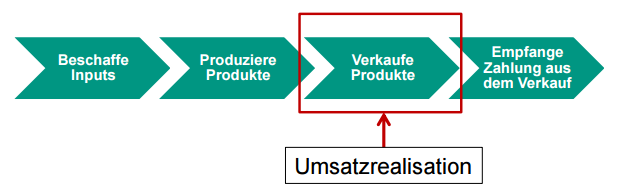
\includegraphics[scale=.5]{umsatzrealisation.png}
\end{center}

\subsection{Matching principle}

Wann sollen Aufwendungen in die Gewinnberechnung einfließen? \\
Das Matching Principle sieht vor, dass Aufwendungen in die
Gewinnberechnung für diejenige Periode einfließen, in der die Erträge, die
diese verursachen, als realisiert gelten.
So fließen die Erträge und ihre verursachten Aufwendungen in den Gewinn
derselben Periode ein.
Es ist dabei nicht entscheidend, dass in dieser Periode auch eine
aufwandsverbundene Auszahlung erfolgt.
Beispiel: Aufwendungen für die Produktion von Produkten fließen dann in die
Gewinnberechnung ein, wenn die Produkte verkauft werden und der Umsatz
realisiert wird.

\section{Jahresabschluss und Geschäftsbericht}

Es gibt zwei Verfahren der GuV-Aufstellung:

\subsection{Umsatzkostenverfahren}

Umsatzerlöse - Umsatzaufwand = Brutto-Ergebnis vom Umsatz \\
+ Sonstige Erträge - Vertriebsmittel - Allgemeiner Verwaltungsaufwand - Sonstige Aufwendungen = Ergebnis der betrieblichen Tätigkeit \\
+ Finanzerträge - Finanzierungsaufwendungen = Periodenergebnis vor Steuern\\
 - Ertragssteueraufwand = Periodengewinn/verlust 

\subsection{Gesamtkostenverfahren}

Umsatzerlöse + Sonstige Erträge +/- Bestandveränderungen fertiger und unfertiger Erzeugnisse - Materialaufwand - Personalaufwand - Planmäßige Abschreibungen - Sonstige Aufwendungen = Ergebnis der betrieblichen Tätigkeit \\
+ Finanzerträge - Finanzierungsaufwendungen = Periodenergebnis vor Steuern\\
 - Ertragssteueraufwand = Periodengewinn/verlust 

\subsection{Kapitalflussrechnung}

Cash Flow aus laufender Geschäftstätigkeit
+ Cash Flow aus der Investitionstätigkeit
+ Cash Flow aus der Finanzierungstätigkeit
= Zahlungswirksame Veränderung des Finanzmittelbestandes

\subsubsection{Cashflow aus laufender Geschäftstätigkeit}

\textbf{Direkte Methode:}\\
Cash Flow aus laufender Geschäftstätigkeit = Operative Einzahlungen - Operative Auszahlungen \\
\textbf{Indirekte Methode:}\\
Cash Flow aus laufender Geschäftstätigkeit = \\
Periodenergebnis vor außerordentlichen Posten\\
+/- Abschreibungen/Zuschreibungen auf Gegenstände des Anlagevermögens\\
+/- Zunahme/Abnahme der Rückstellungen\\
+/- Sonstige zahlungsunwirksame Aufwendungen/Erträge\\
-/+ Gewinn/Verlust aus dem Abgang von Gegenstanden des Anlagevermögens\\
-/+ Zunahme/Abnahme der Vorräte, der Forderungen aus Lieferungen und Leistungen sowie anderer Aktiva, die nicht der Investitions- oder Finanzierungstätigkeiten zuzuordnen sind \\
+/- Zunahme/Abnahme der Verbindlichkeiten aus Lieferungen und Leistungen sowie anderer Passiva, die nicht der Investitions- oder Finanzierungstätigkeiten zuzuordnen sind\\
+/- Ein- und Auszahlungen aus außerordentlichen Posten\\

\section{Bilanzierung}

\subsection{Fair value}

Als fair value wir derjederjenige Preis bezeichnet, den der Vermögenswert beim jetzigen Verkauf erbringen würde.
Der bestmögliche fair value ist der Marktpreis einess/r vergleichbaren Transaktion.


\end{document}
